\chapter{Categories, functions, and constructions}


\epigraph{Watch how children play\\
with blocks: subject, verb, object --\\
towers built on trust.}{}

\section{Subjects} \label{sec:subjects2}
In everyday discourse, the term \textsc{subject}\is{subject (Subj)!characteristics of|(}\is{subject (Subj)!position relative to verb|(}\is{subject (Subj)!denotation}\is{subject (Subj)!and active vs passive}\is{subject (Subj)!pronoun case} refers to topics\is{topic!vs subject (syntactic)} of discussion, areas of study, focal points in visual arts, and even roles in sociopolitical contexts. However, within the realm of syntax, subjects take on a specialized technical meaning denoting one kind of function of a phrase (remember that one-word phrases are common), a special sub-type of complement\is{complement, complementation}.

At the risk of sounding repetitive, I will reiterate that there are no perfect definitions (see Section \ref{sec:conditions}), but we can provide a set of characteristics.

While Section \ref{sec:subjects} introduced the basic syntactic roles and behaviors of subjects, here we'll consider some exceptions and variations. The subject function in a clause typically exhibits the following characteristics:

\begin{itemize}[noitemsep]
    \item The subject is a phrase (often an NP, but can also be a clause, VP, or even PP) that occurs before the head verb in a standard declarative clause.
    \item It appears after an auxiliary verb in most interrogative clauses.
    \item Semantically, the subject often denotes the agent/actor\is{subject (Subj)!denotation!agent/actor} in active clauses, but can also represent the patient/recipient\is{subject (Subj)!denotation!patient/recipient} in passive\is{passive!and subject--object alternation} constructions or an instrument\is{subject (Subj)!denotation!instrument} or other role.\footnote{A \textsc{patient} is the entity that undergoes an action or is affected by it, as opposed to the agent who performs the action. For example, in \textit{The dog chased the cat}, the cat is the patient.}
    \item It's omitted or found in the \textit{by}-phrase of any related passive clause.
    \item If the subject is a pronoun, it's typically in the nominative case\is{case!and subjects}\is{case!nominative case} (see Table \ref{tab:pronouns}).
    \item The subject is licensed by the head verb, with different verbs allowing different types of subjects based on their semantic properties.
    \item It usually controls the person and number agreement\is{agreement!subject--verb|(}\is{subject (Subj)!subject--verb agreement|(} of a present-tense verb, though features like collective vs plural interpretation can impact agreement patterns.
\end{itemize}

To illustrate these characteristics more concretely, consider the following examples.

\subsection{Some examples}

\subsubsection*{Position of subjects relative to verbs}
In each example, the subject is underlined and its verb is double underlined. 

\ea
    \ea[]{\textit{\uline{They} \uuline{greeted} us.}}
    \ex[]{\textit{\uline{The cat} \uuline{sleeps} on the porch.}}
    \ex[]{\textit{In the garden, \uline{the flowers} \uuline{bloom} brightly.}}
    \ex[]{\textit{Quickly, \uline{I} \uuline{need} to go to the store.}}
    \ex[]{\textit{\uline{Water} \uuline{is} boiling on the stove.}}
    \ex[]{\textit{\uuline{Did} \uline{you} meet him at noon?}}
    \ex[]{\textit{Without delay, \uline{the meeting} \uuline{was} adjourned.}}
    \ex[]{\textit{\uline{The book} \uuline{lies} forgotten on the shelf.}}
    \ex[]{\textit{Quietly, \uline{the night} \uuline{falls}.}}
    \ex[]{\textit{Guys, \uuline{can} \uline{you} help me?}}
    \ex[]{\textit{If \uline{it} \uuline{works}, \uline{I}'\uuline{ll} be pleased.}}
    \ex[]{\textit{\uline{She} \uuline{likes} it when \uline{everything} \uuline{works} out.}}
    \z
\z

Consider, though, the following constructions (discussed in Section \ref{sec:preposing}).

\ea
    \ea[]{\textit{Up \uuline{popped} \uline{the toast}}}
    \ex[]{\textit{In the pond \uuline{live} \uline{thousands of tadpoles}.}}
    \z
\z

\subsubsection*{Category of subjects}\is{subject (Subj)!characteristics of|)}\is{subject (Subj)!position relative to verb|)}\is{subject (Subj)!categories functioning as|(}
In the examples above, all the subjects are regular NPs\is{noun, noun phrase (NP)!functions of NP!subject}. Here are some other. 

\ea
    \ea[]{\textit{\uline{Whether it does} is unclear.}\hfill[Clause]}
    \ex[]{\textit{\uline{That the stars are visible} surprises me.}\hfill[Clause]}
    \ex[]{\textit{Here, \uline{to believe wholeheartedly} is not always a virtue.}\hfill[Infinitival VP]\is{verb, verb phrase (VP)!as subject}}
    \ex[]{\textit{\uline{Studying grammar} seems useful.}\hfill[Participial VP]}
    \ex[]{\textit{In the library, \uline{reading quietly} is expected.}\hfill[Participial VP]}
    \ex[]{\textit{\uline{What you know} can help.}\hfill[Relative NP]}
    \ex[]{\textit{\uline{Who you see} isn't our concern.}\hfill[Relative NP]}
    \ex[]{\textit{\uline{Eager} is good.}\hfill[AdjP]\is{adjective, adjective phrase (AdjP)!as subject}}
    \ex[]{\textit{\uline{After 2:00} is too late.}\hfill[PP]\is{preposition, preposition phrase (PP)!functions of PP!subject}}
    \z
\z

\subsubsection*{Denotation} \label{sec:subject-denotation}
Although the (syntactic) subject is typically the (semantic) topic\is{topic!how to nominate}, it needn't be. We can nominate other topics with phrases such as \textit{when it comes to~\dots}, \textit{as for~\dots}, \textit{as far as~\dots~goes}, \textit{speaking of~\dots}, etc., in which cases, the topic of the sentence would not be its subject unless they happen to refer to the same thing (e.g., \textit{As for \uuline{me}, \uline{I} hadn't thought about it}).

\ea
    \ea Subjects denoting actors/agents:
        \ea[]{\textit{As for the rest, \uline{I}'ll leave them here.}}
        \ex[]{\textit{\uline{Who} cooked dinner?}}
        \ex[]{\textit{\uline{The driver} got up and opened the window.}}
        \z
    \ex Subjects denoting patients/recipients:
        \ea[]{\textit{\uline{The ball} was hit over the fence, and \uline{the window} got smashed.}\is{passive!be vs get@\textit{be} vs \textit{get}}}
        \ex[]{\textit{\uline{We} were given a choice.}}
        \ex[]{\textit{\uline{They} got a package.}}
        \z
    \ex Subjects denoting instruments and other roles:
        \ea[]{\textit{\uline{The computer} helped me speed up the analysis.}}
        \ex[]{\textit{\uline{Grammar} is part of language.}}
        \ex[]{\textit{\uline{Studying grammar} seems useful.}}
        \ex[]{\textit{\uline{These things} can hurt.}}
        \ex[]{\textit{\uline{Who you're friends with} isn't our concern.}}
        \ex[]{\textit{Here, \uline{to believe wholeheartedly} is not always a virtue.}}
        \ex[]{\textit{\uline{That the stars are visible} surprises me.}}
        \ex[]{\textit{\uline{They}'re at school.}}
        \ex[]{\textit{\uline{The broom} fell over.}}
        \ex[]{\textit{\uline{It} always surprises me that I can see the stars here.}}
        \z
    \z
\z\is{subject (Subj)!categories functioning as|)}

\subsubsection*{Active vs passive}
Not every active clause has a passive counterpart, but when one exists, the subject of the active clause is typically omitted in the passive, though it can appear in an optional \textit{by} PP. 

\ea\label{ex:passive-no-by}
    \ea[]{\textit{\uline{I} dropped it.} \rightarrow~\textit{It was dropped.}}
    \ex[]{\textit{\uline{We} told them.} \rightarrow~\textit{They were told.}}
    \ex[]{\textit{\uline{Anybody} can use the room.} \rightarrow~\textit{The room can be used by anybody.}}
    \z
\z

In (\ref{ex:passive-no-by}c), don't think that \textit{anybody} remains the subject in the passive clause. Instead, \textit{the room} becomes the subject, and \textit{anybody} is the object in the \textit{by} PP.

\subsubsection*{Pronoun case}
Pronoun subjects are overwhelmingly nominative case: \textit{I}, \textit{you}, \textit{he}, \textit{she}, \textit{we}, \textit{they}\is{case!accusative case}\is{case!genitive case}. See the examples above. In a more formal participial constructions, the possessive may be used; the accusative is now commoner, but may sound too informal:  

\ea
    \ea[]{\textit{\ob \uline{Their}/\uline{Them} asking us\cb~is a huge honor.}}
    \ex[]{\textit{\ob \uline{His}/\uline{Him} hiding it\cb~was a problem.}}
    \ex[]{\textit{\ob \uline{Your}/\uline{You} saying so\cb~does not make it true.}}
    \z
\z

In a \textit{to} infinitival VP, the subject appears in the accusative case after \textit{for}. \textit{It's not for \uline{me} to say.} \textit{It's time for \uline{us} to go.} \textit{I've been waiting for \uline{them} to ask.} \textit{Is there a way for \uline{him} to try again.}

\subsubsection*{Licensing}\is{subject (Subj)!licensing|(}
The subject is a kind of complement licensed by the head verb\is{licensing!of subjects by verb|(}, but instead of following the verb inside the VP, as most such complements do, it typically appears inside the clause but outside of the VP: Subject $+$ Head VP.

Verbs almost universally license NP subjects. The other types of subjects are sensitive to selection by the licensing verbs, and only a few verbs license those subjects.

A \textit{whether} clause is licensed as the subject by only a few lexical verbs such as \textit{affect}, \textit{bother}, \textit{concern}, \textit{depend}, \textit{influence}, \textit{interest}, \textit{matter}, and \textit{worry}\is{polarity (positive vs negative)!of \textit{whether}-clause subjects}. Moreover, this construction is mildly polarity sensitive, preferring negative contexts (see \ref{sec:polarity-items}). Compare 

\ea
    \ea[]{\textit{\uline{Whether it is true or not} doesn't worry me much.}\hfill[negative]}
    \ex[\textsuperscript{?}]{\textit{\uline{Whether it is true or not} worries me.}\hfill[positive]}
    \ex[*]{\textit{\uline{Whether it rained last night} explains the flood.}\hfill[unlicensed]}
    \z
\z
    
Weather verbs, along with {\textit{be}} in weather contexts, license dummy \textit{it}\is{dummy pronoun} (see Section \ref{sec:dummy}). 

\ea
    \ea[]{\textit{It snows here most of the time.}}
    \ex[]{\textit{It's raining.}}
    \ex[]{\textit{It should be sunny tomorrow.}}
    \z
\z

Verbs of appearance and existence license dummy \textit{there}: 

\ea
    \ea[]{\textit{There's a pen in the drawer.}}
    \ex[]{\textit{There seem to be three options.}}
    \ex[]{\textit{There appeared a gossamer web.}}
    \ex[*]{\textit{There disappeared a gossamer web.}}
    \z
\z\is{licensing!of subjects by verb|)}\is{subject (Subj)!licensing|)}

\subsubsection*{subject--verb agreement for number and person}
Agreement is mainly an issue with present-tense verbs for third-person singular subjects. It also affects the various forms of \textit{be} in both the present and past tenses. 

\ea
    \ea[]{\textit{\uline{I}'m here.}}
    \ex[]{\textit{\uline{We}'re here.}}
    \ex[]{\textit{\uline{She}'s here.}}
    \ex[]{\textit{\uline{You} seem kind.}}
    \ex[]{\textit{\uline{It} seems good.}}
    \ex[]{\textit{\uline{The change} works well.}}
    \ex[]{\textit{\uline{The changes} work well.}}
    \ex[]{\textit{\uline{Mia and Iman} go to U of T.}\is{agreement!and coordination}}
    \z
\z

If you're wondering whether a particular NP is the subject, try changing its number and person\is{agreement!as a test for subjecthood} (see also Box \ref{box:finding-subject}). For example, let's say you're wondering about the subject in \textit{of all the girls who I have loved, \dots}. You've decided it could be \textit{all the girls} (third-person plural), \textit{who} (third-person singular), or \textit{I} (first-person singular). You can try the following: \textit{of the girl who I have loved} (no change in agreement), \textit{of all the girls I have loved} (no change in agreement), and \textit{of all the girls who he has loved} (\textit{have} changes to \textit{has}). This is good evidence that the subject is \textit{I}.

Unfortunately, it's not a perfect test. Other elements may control agreement\is{agreement!complications and exceptions}. This can be some dependent in the subject, as in \textit{\uline{A number of }\uuline{people} have arrived.} Or with dummy \textit{there}\is{dummy pronoun!and subject--verb agreement}, it's the complement of the head verb: \textit{\uline{There} was \uline{something} on the floor.} \textit{\uline{There} were \uline{some things} on the floor.}\is{agreement!subject--verb|)}\is{subject (Subj)!subject--verb agreement|)}

\subsection{Subject dropping}\label{sec:subject-dropping}\is{subject (Subj)!dropping|(}\is{cross-linguistic influence}
In many languages it is common, and even sometimes obligatory, to omit the subject. For instance, Italian\il{Italian} examples like (\ref{ex:abbiamo}) lack a subject, but the verb form tells you that it's first-person plural\is{subject (Subj)!dropping!in other languages (Italian, Japanese)}.

\ea \label{ex:abbiamo}
    \gll \textit{Abbiamo} \textit{iniziato} \textit{a} \textit{studiare} \textit{la} \textit{grammatica} \\
    have-\textsc{1st-pl} started to study the grammar \\
        \glt `We started studying grammar'
\z
    
Japanese\il{Japanese} often omits a subject, and without either number or person marking on the verb, the interpretation is entirely contextual.

\ea
    \ea \label{ex:tabeta}
    \glll \textit{食べた} \\
    tabeta \\
    eat-\textsc{past} \\
    \glt `(I) Ate' (or somebody else)
    \ex \label{ex:ikitai}
    \glll \textit{行きたい?} \\
    ikitai \\
    go-\textsc{pres-desirative} \\
    \glt `Do (you) want to go?' (or somebody else)
    \z
\z

English subjects, though, are generally considered to be obligatory. Certainly, in formal writing, every main clause~-- apart from imperatives~-- has a subject. But in speech, even if the verb doesn't tell you who the subject is, it's often clear that it's the speaker or the addressee. In such cases, it's common to drop the subject \textit{I} in English too, as in (\ref{ex:first-person-drop})\is{subject (Subj)!dropping!in English}.

\ea  \label{ex:first-person-drop}
    \ea[]{\textit{Hope not.}}
    \ex[]{\textit{Think so.}}
    \ex[]{\textit{Dunno.}}
    \ex[]{\textit{Got it.}}
    \ex[]{\textit{Can't find my keys.}}
    \ex[]{\textit{Love this song.}}
    \ex[]{\textit{Went to the store earlier.}}
    \ex[]{\textit{Oh! See what you mean.}}
    \ex[]{\textit{Woke up late, ran out the door, and missed the bus.}}
    \z
\z

For the addressee, it's also common to drop the subject in aux-first interrogatives, although it's not exactly the same thing because you can't drop \textit{you} without also dropping the auxiliary verb, as in (\ref{ex:second-person-drop}).

\ea  \label{ex:second-person-drop}
    \ea[]{\textit{Feeling OK?}}
    \ex[]{\textit{Think this looks good?}}
    \ex[]{\textit{Ever been to Paris?}}
    \ex[]{\textit{Know what I mean?}}
    \ex[]{\textit{Want some coffee?}}
    \ex[]{\textit{Need a hand with that?}}
    \z
\z

In fact, it's possible to drop just the auxiliary and use \textit{you} in each example in (\ref{ex:second-person-drop}).

Even third-person examples can work if the context is right, as in (\ref{ex:third-person-drop}).
\ea  \label{ex:third-person-drop}
    \ea[]{A: \textit{Where did Ying go?} B: \textit{Went to the store.}}
    \ex[]{A: \textit{Why isn't Patel playing today?} B: \textit{Got injured during practice.}}
    \ex[]{A: \textit{Did the kids finish their homework?} B: \textit{Finished it ages ago.}}
    \z
\z

Even in main clauses, third-person subjects are regularly dropped when the clause is the second or subsequent coordinate in a coordination\is{coordination}, although these are arguably coordinated VPs. However you think about it, constructions like those in (\ref{sec:coord-drop}) are very common in English.

\ea \label{sec:coord-drop}
    \ea[]{\textit{They turned around and \ob they \cb~made their way back.}}
    \ex[]{\textit{I opened it and \ob I \cb~took a look.}}
    \ex[]{\textit{A nurse came into the room and \ob she \cb~asked Bill how he was doing}}
    \z
\z

What this shows is that subject dropping is actually quite common when the subject is easily understood. In some languages, like Italian\il{Italian}, it's easier because of verb endings. In others, like Japanese\il{Japanese} and Korean\il{Korean}, it's just expected that the listener will follow the topic closely and work it out. There's more about this in  Section \ref{sec:ellipsis}.

It's common for English-language teachers to insist that their students produce ``full sentences.'' This is misguided and can be confusing. It gives many students the idea that, to be polite, their English needs to sound stiff, natural, and disconnected. If they follow their teachers' admonishments, they may end up seeming more alien than if they used the drop forms\is{subject (Subj)!dropping}.

That said, students commonly drop subjects where no expert English speaker would. This kind of subject dropping is ungrammatical and can be quite confusing to the audience. It should be discouraged when there is an appropriate opportunity for form-focused feedback.

\subsection{Conclusion}
Subjects exhibit a range of characteristics, including their position relative to verbs, the categories that can function as subjects, their typical denotation, their behavior in active and passive constructions, and their role in subject--verb agreement. The topic of subject dropping highlights the differences between English and many other languages, while also showcasing the often-unacknowledged flexibility of subject omission in informal English speech. By examining these properties and considering counter-examples, we can better anticipate the kinds of problems our students will face.\is{subject (Subj)!dropping|)}

\section{Determiners}\is{determiner (Det)|(}\is{determiner (Det)!position in NP|(}
It's time to flip things around. For this section, we'll start with a bunch of examples, and then it will be up to you to draw out the characteristics.

Before we start, though, a quick reminder: \textsc{determinative}\is{determiner (Det)!vs determinative (category)}, like \textsc{adjective}, is a lexical category. \textsc{Determiner}, like \textsc{modifier}, is a syntactic function.

\ea \label{ex:determiners}
    \ea\textit{Hardly \uline{a} day goes by without progress.}
    \ex\textit{I saw him only \uline{a few} days ago.}
    \ex\textit{We've only got \uline{a little} time.} 
    \ex\textit{\uline{All} good people are welcome.} 
    \ex\textit{Do you want \uline{any} fresh coffee?} 
    \ex\textit{\uline{The} other two rooms had windows at \uline{both} ends.} 
    \ex\textit{It happened \uline{each} year.} 
    \ex\textit{\uline{Most} people work about \uline{eight} hours a day.} 
    \ex\textit{\uline{My} new job takes \uline{far less than 40} hours per week.} 
    \ex\textit{\uline{How many} times have I walked down \uline{this} street where you lived?} 
    \ex\textit{\uline{Many more} changes are coming.} 
    \ex\textit{\uline{Neither} definition seems correct.} 
    \ex\textit{There is \uline{almost no} water left.} 
    \ex\textit{Give me \uline{that} book, not \uline{this} one.} 
    \ex\textit{I'm going to take \uline{these} sandwiches for \uline{my} lunch.} 
    \ex\textit{It's different for \uline{us} women.} 
    \ex\textit{\uline{Which} ones do you like?} 
    \ex\textit{Even \uline{your} critics say you're right \uline{this} time.}
    \ex\textit{\uline{Canada's} population is growing quickly.} 
    \ex\textit{He's head of \uline{the World Health Organization's} AIDS program.}
    \z
\z

\begin{enumerate}[noitemsep]
    \item In which phrasal category/ies are determiners dependents?
    \item Where do determiners appear relative to the head?
    \item Where do determiners appear relative to modifiers?
    \item How does number and countability impact the need for a determiner?
    \item What is the role of determiners regarding definiteness?
    \item What kind of agreement do we find for determiners?
    \item What are the phrase types that most commonly function as determiners?
\end{enumerate}

\begin{tcolorbox}[title=Determiners: A brief history\is{determiner (Det)!history of the term}, colback=white]

The very idea that determiners are something distinct from modifiers wasn't recognized until about 1933, at least, not as it applies to English. In his seminal 1933 work \textit{Language}, Leonard Bloomfield\ia{Bloomfield, Leonard} introduced the term \textsc{determiner} to refer to a specific syntactic function performed by what he called ``limiting adjectives.''

~~~~Bloomfield observed that certain noun expressions, such as \textit{house} or \textit{big house}, are ``always accompanied by a determiner'' \citep[203]{bloomfield1984language}. Modifiers, in contrast are optional. This is sort of like an anthropologist realizing that some of these ancient arrowheads they'd known about for hundreds of years were actually spear points.

~~~~Despite almost 100 years having passed since Bloomfield's recognition of determiner as a distinct syntactic function, most pedagogical grammars remain confused on the point. If they use the term, they apply it indistinctly both to the category of determinatives and the function of determiners. It doesn't really matter what terms you use, but it seems very useful to me to maintain terminological hygiene\is{terminological hygiene!as a guiding principle}, which is to say not to use one term for two distinct concepts.

\end{tcolorbox}

\subsection{Position and Ordering within NP}

Determiners appear only in NPs, typically preceding all other dependents within the NP. For example:

\begin{itemize}[noitemsep]
   \item \textit{\uline{the} big red ball}
   \item \textit{\uline{some} really interesting books}
   \item \textit{\uline{every} student in the class}
\end{itemize}\is{determiner (Det)!position in NP|)}

There are cases where there is a predeterminer modifier, but these are rare and I've never been asked about them by ESL students. Nevertheless, if only for the sake of completeness, it's worth mentioning that \textit{all} functions as just such a predeterminer modifier in \textit{all the books}, with \textit{the} functioning as the determiner.

\subsection{Categories functioning as determiners}\is{determiner (Det)!categories functioning as determiners|(}

The determiner function is a determinative phrase (DP)\is{determinative, determinative phrase (DP)!as determiner} in the vast majority of cases. The remaining cases are almost all possessive NPs\is{determiner (Det)!categories functioning as determiners!possessive NP}, either pronouns like \textit{my}, \textit{their}, \textit{whose}, etc. or NPs headed by common or proper nouns, such as the last two examples in (\ref{ex:determiners}).

A possessive NP often includes its own determiner, as in the two examples in Figure \ref{fig:det-det}. \textit{My uncle's dog} has \textit{my} as the determiner in the NP \textit{my uncle's}, which, in turn, functions as determiner in the larger NP. In \textit{this morning's headlines}, singular \textit{this} is the determiner in the singular NP \textit{this morning's}, not in the plural NP *\textit{this headlines}.

\begin{figure}
    \centering
    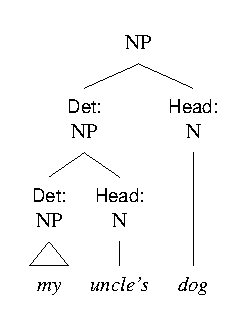
\includegraphics[width=0.315\linewidth]{figures/my-uncles-dog.pdf}
    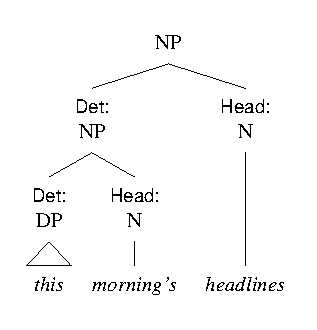
\includegraphics[width=0.4\linewidth]{figures/this-mornings-headlines.pdf}
    \caption{Tree diagrams showing nested determiner structures in \textit{my uncle's dog} and \textit{this morning's headlines}.}
    \label{fig:det-det}
\end{figure}

Beyond these possessive structures, certain interrogative and relative words~-- the determinatives \textit{which} and \textit{what}, and the pronoun \textit{whose}~-- can also function as determiners (See Sections \ref{sec:interrogative-phrases} \& \ref{sec:focused-articulated}).\is{determiner (Det)!categories functioning as determiners|)}

\subsection{Agreement and Concord}\is{agreement!determiner--head}\is{determiner (Det)!agreement and concord|(}

Determiners often exhibit agreement with the head noun in terms of number and, in some cases, gender. This phenomenon is known as concord.

\subsubsection{Number Agreement}\is{determiner (Det)!agreement and concord!number agreement}
Determiners typically agree with the head noun in terms of number:

\begin{itemize}[noitemsep]
   \item Singular: \textit{the book}, \textit{this car}, \textit{my friend}
   \item Plural: \textit{the books}, \textit{these cars}, \textit{my friends}
\end{itemize}

Some determiners, such as \textit{some}, \textit{any}, and \textit{no}, can be used with both singular and plural nouns without any change in form.

\subsubsection{Gender Agreement}\is{determiner (Det)!agreement and concord!gender agreement}
In English, gender agreement is not as prevalent as in many other languages. However, there are a few cases where determiners agree with the natural gender of the referent:

\begin{itemize}[noitemsep]
   \item Masculine: \textit{his book}
   \item Feminine: \textit{her book}
   \item Neuter: \textit{its book}
\end{itemize}

It's important to note that gender agreement in English is primarily limited to personal pronouns and possessive determiners. Most determiners do not exhibit gender distinctions.\is{determiner (Det)!agreement and concord|)}\is{determiner (Det)|)}

\section{Objects}\is{object (Obj)|(}

Objects are a special kind of complement\is{object (Obj)!vs complement} in VPs and PPs. They're overwhelmingly NPs\is{noun, noun phrase (NP)!functions of NP!object}, and they differ from other types of VP complements in that the same NP can usually function as the subject in the passive construction\is{object (Obj)!and passive alternation|(}\is{passive!and subject--object alternation}, though not always as (\ref{ex:cant-passive-obj}) shows.

\ea
    \ea[]{\textit{Somebody reported \uline{a theft}.}\hfill[\textsc{object}]}
    \ex[]{\textit{\uline{A theft} was reported.}\hfill[\textsc{subject in passive}]}
    \z
\z
\ea \label{ex:cant-passive-obj}
    \ea[]{\textit{I weigh \uline{seventy kilograms}.}\hfill[\textsc{object}]}
    \ex[*]{\textit{\uline{Seventy kilograms} is weighed {\op}by me{\cp}.}\hfill[\textsc{subject in passive}]}
    \z
\z
\ea
    \ea[]{\textit{It became \uline{a problem}.}\hfill[\textsc{non-object complement}]}
    \ex[*]{\textit{\uline{A problem} was become.}\hfill[\textsc{subject in passive}]}
    \z
\z

Most objects in PPs\is{object (Obj)!object of preposition} can't undergo this same alternation, though it is sometimes possible.

\ea
    \ea[]{\textit{She went \ob to \uline{Toronto}\cb.}\hfill[\textsc{object in PP}]}
    \ex[*]{\textit{\uline{Toronto} was gone \ob to \cb.}\hfill[\textsc{subject in passive}]}
    \z
\z
\ea
    \ea[]{\textit{Someone broke {\ob}into \uline{the house}\cb.}\hfill[\textsc{object in PP}]}
    \ex[]{\textit{\uline{The house} was broken {\ob}into \cb.}\hfill[\textsc{subject in passive}]}
    \z
\z\is{object (Obj)!and passive alternation|)}

Verbs and prepositions that take objects are called \textsc{transitive}\is{transitivity}\is{licensing!of objects (transitivity)}, while those that don't are \textsc{intransitive}. Some verbs are \textsc{ditransitive}\is{transitivity}~-- they take two objects, the first being the \textsc{indirect object}\is{object (Obj)!indirect}, and the second being the \textsc{direct object}\is{object (Obj)!direct}.

\ea
    \ea[]{\textit{I gave \uline{them}}\textsubscript{ indirect}\textit{ \uline{the books}}\textsubscript{ direct}\textit{.}\hfill[\textsc{two objects}]}
    \ex[]{\textit{\uline{They} were given the books.}\hfill[\textsc{indir obj becomes subj in passive}]}
    \ex[]{\textit{\uline{The books} were given to them.}\hfill[\textsc{dir obj becomes subj in passive}]}
    \z
\z\is{object (Obj)|)}

\section{Other complements}\is{complement, complementation!vs modifier|(}

Section \ref{sec:verb-complementation} deals with complements in VPs\is{complement, complementation!in clause/VP} and Section \ref{sec:PP-complementation} with complements in PPs\is{complement, complementation!in PP}, but other phrases also allow complements. Here we'll examine complementation in noun phrases and adjective phrases, which were only briefly addressed in Chapter \ref{ch:categories}.

\subsection{Complements in noun phrases}\is{complement, complementation!in NP|(}

Noun phrases can take several types of complements, which differ from modifiers in being more tightly integrated with the head noun and often corresponding to arguments of related verbs\is{licensing!of complements by head}.

\subsubsection{PP complements}\is{complement, complementation!in NP!PP complements}

Many nouns take PP complements, often with specific prepositions. This is particularly common with deverbal nouns (nouns derived from verbs), where the PP complement often corresponds to the complement of the related verb:

\ea
    \ea[]{\textit{her belief \uline{in ghosts}}\hfill[cf. believe in ghosts]}
    \ex[]{\textit{their reliance \uline{on fossil fuels}}\hfill[cf. rely on fossil fuels]}
    \ex[]{\textit{the attack \uline{on the fortress}}\hfill[cf. attack the fortress]}
    \z
\z

\noindent When the verb licenses a direct object, the related noun usually licenses an \textit{of} PP.

\ea
    \ea[]{\textit{management \uline{of the city}}\hfill[cf. manage the city]}
    \ex[]{\textit{the examination \uline{of evidence}}\hfill[cf. examine evidence]}
    \ex[]{\textit{their collection \uline{of artifacts}}\hfill[cf. collect artifacts]}
    \z
\z

\noindent Other nouns select PP complements unrelated to any verbal source:

\ea
    \ea[]{\textit{a solution \uline{to the problem}}}
    \ex[]{\textit{access \uline{to healthcare}}}
    \ex[]{\textit{an addiction \uline{to sugar}}}
    \z
\z

\subsubsection{Clausal and VP complements}\is{complement, complementation!in NP!clausal complements}\is{complement, complementation!in NP!VP complements}

Some nouns, particularly those related to speech and mental states, can take clausal complements:

\ea
    \ea[]{\textit{the claim \uline{that Earth is flat}}}
    \ex[]{\textit{her suggestion \uline{that we leave early}}}
    \z
\z

\noindent Others, also related to speech and mental states, can take \textit{to}-infinitival VP complements.
\ea
    \ea[]{\textit{the desire \uline{to succeed}}}
    \ex[]{\textit{the decision \uline{to resign}}}
    \z
\z

\noindent Again, the type of complement often mirrors what's possible with the related verb:

\ea
    \ea[]{\textit{She claimed \uline{that Earth is flat}} $\rightarrow$ \textit{the claim \uline{that Earth is flat}}}
    \ex[]{\textit{They decided \uline{to resign}} $\rightarrow$ \textit{the decision \uline{to resign}}}
    \z
\z\is{complement, complementation!in NP|)}

\subsection{Complements in adjective phrases}\is{complement, complementation!in AdjP|(}

Adjectives can also take various types of complements, which differ from modifiers in being selected by specific adjectives.

\subsubsection{PP complements}\is{complement, complementation!in AdjP!PP complements}

Many adjectives select specific prepositions:

\ea
    \ea[]{\textit{afraid \uline{of spiders}}}
    \ex[]{\textit{similar \uline{to his brother}}}
    \ex[]{\textit{proud \uline{of her achievements}}}
    \ex[]{\textit{dependent \uline{on fossil fuels}}}
    \ex[]{\textit{interested \uline{in linguistics}}}
    \z
\z

The choice of preposition is rarely predictable and needs to be learned with each adjective. Compare:

\ea
    \ea[]{\textit{interested \uline{in} grammar} vs \textit{keen \uline{on} grammar}}
    \ex[*]{\textit{keen \uline{in} grammar} vs *\textit{interested \uline{on} grammar}}
    \z
\z

\subsubsection{Clausal and VP complements}\is{complement, complementation!in AdjP!clausal complements}\is{complement, complementation!in AdjP!VP complements}

Some adjectives can take clausal and VP complements. Again, these tend to be those related to speech or mental states:

\ea
    \ea[]{\textit{happy \uline{that you came}}}
    \ex[]{\textit{certain \uline{that it would work}}}
    \ex[]{\textit{eager \uline{to help}}}
    \ex[]{\textit{busy \uline{preparing}}}
    \z
\z\is{complement, complementation!in AdjP|)}\is{complement, complementation!vs modifier|)}


\subsection{Conclusion}

While verb complementation may be more familiar to students, the complement system extends beyond VPs to other major phrasal categories. Both NPs and AdjPs employ a variety of complementation strategies to express relationships between heads and their arguments. The key distinction from modifiers lies in complements being selected by specific heads and often being obligatory for the phrase's grammaticality or complete meaning. Understanding these patterns helps explain both the syntactic structure of English phrases and the semantic relationships between their components.

\section{Modifiers} \label{sec:modifiers}\is{modification, modifier|(}\is{modification, modifier!vs complement|(}

Modifiers are dependents that augment, qualify, or restrict the meaning of their head. Unlike complements, they aren't licensed by specific heads and are generally optional. Let's look at some examples with the modifiers underlined:

\ea\label{ex:modifier-types}
   \ea[]{\textit{The {\ob}\uline{tall} woman \uline{in red}{\cb} {\ob}smiled \uline{broadly}{\cb}.}}
   \ex[]{\textit{The {\ob}\uline{surprisingly difficult} exam \uline{we took}{\cb} stressed everyone {\ob}\uline{quite} badly{\cb}.}}
   \ex[]{\textit{She {\ob}works {\ob}\uline{very} efficiently{\cb} \uline{in the morning}{\cb}.}}
   \ex[]{\textit{The {\ob}\uline{old} book \uline{on the shelf} \uline{that I mentioned}{\cb} belongs to Pat.}}
   \z
\z

Several key characteristics define modifiers:

\begin{itemize}[noitemsep]
   \item They're typically optional~-- removing them may affect meaning but usually preserves grammaticality (but consider \textit{poorly} in \textit{The results compare poorly to last year's.})
   \item Multiple modifiers can stack up with the same head
   \item They can appear in various positions relative to the head
   \item Different phrasal categories can function as modifiers
   \item Unlike complements, you can usually add more 
\end{itemize}\is{modification, modifier!vs complement|)}

\subsection{Position of modifiers}\is{modification, modifier!position of|(}

The position of modifiers varies by the category of both the modifier and the phrase it's modifying. In NPs\is{modification, modifier!in NP}, we find both premodifiers (before the head) and postmodifiers (after the head):

\ea\label{ex:np-modifiers}
   \ea[]{\textit{two \uline{bright} \uline{red} cars}\hfill[premodifiers]}
   \ex[]{\textit{the book \uline{on the table} \uline{with the blue cover}}\hfill[postmodifiers]}
   \ex[]{\textit{the \uline{young} student \uline{from Toronto}}\hfill[pre- and postmodifiers]}
   \z
\z

In clause structure\is{modification, modifier!in clause/VP}, modifiers can generally appear in various positions:

\ea\label{ex:vp-modifiers}
   \ea[]{\textit{\uline{Quickly}, she answered the phone.}\hfill[initial]}
   \ex[]{\textit{She \uline{quickly} answered the phone.}\hfill[pre-verbal]}
   \ex[]{\textit{She answered the phone \uline{quickly}.}\hfill[final]}
   \z
\z

Some modifiers have strong preferences for certain positions though. Compare:

\ea\label{ex:modifier-position}
   \ea[]{\textit{The students \uline{merely} wanted to help.}}
   \ex[?]{\textit{The students wanted to help \uline{merely}.}}
   \z
\z\is{modification, modifier!position of|)}

\subsection{Categories functioning as modifiers}\is{modification, modifier!categories functioning as|(}

Different phrasal categories can function as modifiers:

\begin{itemize}[noitemsep]
   \item AdjPs typically function as modifiers in NPs\is{adjective, adjective phrase (AdjP)!as modifier}: \textit{the \uline{happy} child}
   \item AdvPs can modify in any type of phrase except NPs\is{adverb, adverb phrase (AdvP)!as modifier}: \textit{\uline{very} quickly}
   \item PPs can function as modifiers in most types of phrases: \textit{the book \uline{on the shelf}}
   \item Relative clauses function mostly as modifiers in NPs: \textit{the book \uline{that I bought}}
   \item Even NPs can sometimes function as modifiers\is{noun, noun phrase (NP)!functions of NP!modifier}: \textit{It snowed \uline{last week}, I met her \uline{this morning}}, an \uline{old folks'} home, the \uline{faculty} office.
   \item And DPs\is{determinative, determinative phrase (DP)!as modifier}: \textit{It wasn't \uline{all that} difficult, We drank \uline{almost all} the water.}
\end{itemize}

\begin{table}[h]
\centering
\begin{tabular}{lcccccc}
\hline
Often Modify $\rightarrow$ & NP & AdjP & AdvP & PP & VP & DP \\
\hline
\textbf{NP} & ✔ &~-- &~-- &~-- & ✔ &~-- \\
\textbf{AdjP} & ✔ &~-- &~-- &~-- &~-- &~-- \\
\textbf{AdvP} &~-- & ✔ & ✔ & ✔ & ✔ & ✔ \\
\textbf{PP} & ✔ & ✔ & ✔ & ✔ & ✔ & ✔ \\
\textbf{Relative Clause} & ✔ &~-- &~-- &~-- &~-- &~-- \\
\textbf{DP} &~-- & ✔ & ✔ &~-- & ✔ &~-- \\
\hline
\end{tabular}
\caption{Phrase Types as Modifiers}
\label{tab:modifiers}
\end{table}\is{modification, modifier!categories functioning as|)}

\subsubsection{Measure phrases}\is{modification, modifier!measure phrase}

A number of prepositions and adjectives take measure-phrase modifiers:
\ea
    \ea[]{\textit{two years \uline{after the change}}}
    \ex[]{\textit{six months \uline{in}}}
    \ex[]{\textit{three kilometres \uline{down the road}}}
    \ex[]{\textit{two feet \uline{into the air}}}
    \z
    \ea[]{\textit{two meters \uline{tall}}}
    \ex[]{\textit{three years \uline{old}}}
    \ex[]{\textit{six feet \uline{deep}}}
    \ex[]{\textit{ten centimeters \uline{wide}}}
    \z
\z

\subsection{Stacking and ordering}\is{modification, modifier!stacking and ordering}

Multiple modifiers can stack up with the same head, but their order isn't random. In NPs, premodifying adjectives tend to follow patterns based on their semantic type:

\ea\label{ex:adj-order}
   \ea[]{\textit{The \uline{lovely} \uline{old} \uline{brass} lamp}\hfill[opinion-age-material]}
   \ex[\textsuperscript{?}]{\textit{The \uline{brass} \uline{old} \uline{lovely} lamp}\hfill[non-standard order]}
   \z
\z

\noindent Similarly, different types of modifiers in clause structure tend to follow certain ordering principles:

\ea\label{ex:adv-order}
   \ea[]{\textit{She usually works \uline{efficiently} \uline{in the morning} \uline{at the office}.}}
   \ex[\textsuperscript{?}]{\textit{She usually works \uline{at the office} \uline{efficiently} \uline{in the morning}.}}
   \z
\z

\subsection{Integrated vs supplementary modifiers}\is{modification, modifier!integrated vs supplementary|(}

A key distinction in modification is between integrated and supplementary modifiers. Integrated modifiers are part of the larger phrase:

\ea\label{ex:restrictive}
   \ea[]{\textit{The student \uline{who scored highest} won a prize.}\hfill[integrated]}
   \ex[]{\textit{The books \uline{on the top shelf} need dusting.}\hfill[integrated]}
   \z
\z

Supplementary modifiers are simply added to the larger utterance with little regard for phrase structure. They're typically set off in speech with a slight pause, and in writing with commas, parentheses, or dashes:

\ea\label{ex:supplement}
    \ea[]{\textit{Pat, \uline{who scored highest}, won a prize.}\hfill[supplementary relative]}
    \ex[]{\textit{The books, \uline{dusty and neglected}, need sorting.}\hfill[supplementary AdjP]}
    \ex[]{\textit{The meeting, \uline{surprisingly}, went well.}\hfill[supplementary AdvP]}
    \z
\z

The distinction between integrated and supplementary modification has important structural consequences. Integrated modifiers can only appear where the phrase structure allows them~-- inside the phrase they're modifying. Supplementary modifiers, by contrast, can appear in various interpolated positions:

\ea\label{ex:supplement-position}
    \ea[]{\textit{The professor, \uline{as everyone knew}, had cancelled class.}}
    \ex[]{\textit{The professor had, \uline{rather unexpectedly}, cancelled class.}}
    \ex[]{\textit{The professor had cancelled class, \uline{as it turned out}.}}
    \z
\z

Moreover, while integrated modifiers can stack up inside a single phrase, supplementary modifiers tend to appear one at a time, each adding a separate comment:

\ea\label{ex:supplement-stack}
    \ea[]{\textit{The \uline{tall} \uline{young} \uline{energetic} teacher...}\hfill[integrated stack]}
    \ex[]{\textit{The teacher, \uline{quite young}, \uline{surprisingly energetic}, arrived.}\\\hfill[supplementary series]}
    \z
\z

In terms of meaning, integrated modifiers help identify or characterize the meaning of their head, while supplementary modifiers add parenthetical information or speaker commentary. This difference is particularly clear with relative clauses:

\ea\label{ex:relative-contrast}
    \ea[]{\textit{Students \uline{who finish early} may leave.}\hfill[integrated - defines subset]}
    \ex[]{\textit{The students, \uline{who finished early}, left.}\hfill[supplementary - adds info]}
    \z
\z\is{modification, modifier!integrated vs supplementary|)}\is{modification, modifier|)}

\section{Constructions}\label{sec:constructions}\is{construction|(}
Language is not just a collection of individual words, and it's not just the words that hold meaning. Consider phrases like \textit{come here}, \textit{think about it}, or \textit{don't touch that}. The form conveys something more than the sum of the word meanings. Try to take a step back and see it in a new light.

First of all, did you notice that the phrases address `you'. If English had evolved a little differently, perhaps \textit{think about it} could mean `we think about it', `she thinks about it', or `they think about it'. In fact, in Japanese\il{Japanese}, for instance, the closest structural translation, dropping the subject, often means `I'll think about it'. But not in English.

For us, the word \textit{you} is absent and yet the directive is aimed at the person being spoken to. It is the form~-- the grammatical structure itself~-- that says `you', and even a slightly different structure~-- \textit{to think about it} or \textit{thinks about it}~-- means something different.

Secondly, I called it a directive, and it absolutely is. This may seem obvious, but the phrase means both `I want you to do this' and, at the same time, means `I believe that our social and contextual relationship is such that I can reasonably expect you to comply'. It includes an element of compulsion (see Section \ref{sec:power}).

The form of \textit{think about it} didn't have to convey a directive. It's close to a request, but not quite. It could, perhaps, have been a declaration, an exclamation, or a question. It could even have been a conditional = `if you think about it'.

This may seem rather implausible to you. You probably wonder how \textit{think about it} could possibly be conditional, and find the notion utterly preposterous. But not only could it convey conditionality, it does when part of a larger construction: \textit{think about it and you'll see what I mean} (= `\uline{if you think about it}, you'll see what I mean').

When linguists speak about \textsc{constructions}, this is what they have in mind: not just some kind of grammatical structure but one that means something, a form--meaning pairing.\is{construction|)}

\subsection{Conditional coordination}\label{sec:conditional-coordination}\is{construction!conditional coordination|(}

One particularly striking example of a construction is the \textit{think about it} example. I'll call this the \textsc{conditional coordination} construction.

\ea\label{ex:conditional-coord}
   \ea[]{\textit{go and you'll regret it}}
   \ex[]{\textit{touch that and you'll burn yourself}}
   \z
\z

What appears on the surface to be simple coordination\is{coordination|(} with \textit{and} actually expresses a conditional relationship: `if you do X, then Y will happen.' The construction requires specific elements to work: the first coordinate must be an imperative and the second must express the predicted consequence. If we alter either requirement, the conditional meaning disappears:

\ea\label{ex:conditional-coord-constraints}
   \ea[]{\textit{Come closer and I'll tell you a secret.}}
   \ex[*]{\textit{You came closer and I'll tell you a secret.}}
   \ex[]{\textit{Come closer and tell me.}\hfill [coordination only]}
   \z
\z

A closely related construction is what Peter \citet{culicover1970one} called the \textit{one more} construction\is{construction!one more@\textit{one more}}, as in \textit{One more comment like that and I'm leaving.} Again, the first coordinate can be interpreted conditionally, as `if you make one more comment like that'.

The conditional-coordination construction is particularly useful for expressing warnings, threats, and promises. Like many constructions, it shows how English grammar can package complex meanings into conventional patterns that go well beyond the literal meanings of the words involved.\is{coordination|)}


\begin{tcolorbox}[title=Another Syntax-Semantics Mismatch]\is{syntax-semantics mismatch!in conditional coordination}
\citet{culicover1997semantic} made a beautiful observation about these constructions: while syntactically the structure appears to be coordination (\textit{and} joining two equal clauses), semantically the first clause is actually subordinate to the second. This explains why \textit{go and you'll regret it} means `if you go, you'll regret it' rather than `I direct you to go and subsequently you will regret it'. This syntax-semantics mismatch is yet one more example of how constructions can encode meaning patterns that diverge from what we might expect from their structure. It's also another reminder: believe in the fallacy of monosemy\is{monosemy!fallacy of}, and you'll regret it (see Section \ref{sec:fallacy-of-monosemy}).\is{fallacy of monosemy}
\end{tcolorbox}\is{construction!conditional coordination|)}

\subsection{Resultative constructions}\is{construction!resultative|(}

In a resultative construction, an NP object and a following phrase express the result of the action denoted by the verb:

\ea\label{ex:resultative}
   \ea[]{\textit{She wiped the table clean.}}
   \ex[]{\textit{He hammered the metal flat.}}
   \ex[]{\textit{It froze the lake solid.}}
   \z
\z

The result phrase is usually an AdjP (as above) but can sometimes be a PP:

\ea\label{ex:resultative-pp}
   \ea[]{\textit{She tied her hair into braids.}}
   \ex[]{\textit{They smoothed the dough to perfection.}}
   \ex[]{\textit{He carved the wood down to size.}}
   \z
\z

Importantly, the object NP must be affected by the action~-- we can't say *\textit{She drove the road flat} or *\textit{He sang the baby hoarse}. The result must also be a plausible outcome of the action~-- *\textit{She painted the wall tall} is odd because painting doesn't cause height change.\is{construction!resultative|)}

\subsection{Light verb constructions}\is{construction!light verb|(}

Light verb constructions combine a verb that is semantically near empty with an NP to express what could often be conveyed by a single verb:

\ea\label{ex:light-verb}
   \ea[]{\textit{take a walk} (`walk')}
   \ex[]{\textit{have a look} (`look')}
   \ex[]{\textit{give a try} (`try')}
   \ex[]{\textit{make a decision} (`decide')}
   \z
\z

When I say \textit{take}, \textit{have}, \textit{give}, and \textit{make} are ``semantically empty'', I mean they appear more for their syntactic properties than for their meaning: Giving money and having it convey very different things, but \textit{give a try} and \textit{have a try} don't. 

The most common light verbs are \textit{take}, \textit{have}, \textit{give}, and \textit{make}. While these constructions might seem redundant, they serve important discourse functions\is{discourse function!of light verb constructions}. Compare:

\ea\label{ex:light-verb-use}
   \ea[]{\textit{I walked in the park yesterday.}}
   \ex[]{\textit{I took a \uline{nice long} walk in the park yesterday.}}
   \z
\z
The light verb construction allows some modification of the event (denoted by the noun \textit{walk} here) more easily than does the simple verb. It also helps manage information structure\is{information structure!and light verb constructions}, as the event noun can more easily serve as given information in subsequent discourse (See Chapter \ref{ch:info-package}).\is{construction!light verb|)}

\subsection{Serial verb constructions}\is{construction!serial verb constructions|(} 

English has a limited but common set of serial-verb constructions where two verbs combine without any coordinator, subordinator, or preposition:

\ea\label{ex:serial}
   \ea[]{\textit{Go get some coffee.}}
   \ex[]{\textit{Come see what I found.}}
   \ex[]{\textit{Run grab your coat.}}
   \z
\z

The first verb is typically one of motion (\textit{go}, \textit{come}, \textit{run}) and the second describes the action to be performed after the motion. Both verbs must be in the same form~-- we can't mix forms like *\textit{went get} or *\textit{go getting}.

These constructions are more restricted in English than in many other languages. They're mainly limited to imperatives and infinitivals:

\ea\label{ex:serial-forms}
   \ea[]{\textit{I'll go get some coffee.}}
   \ex[]{\textit{She made me go get some coffee.}}
   \ex[*]{\textit{I went got some coffee.}}
   \z
\z\is{construction!serial verb constructions|)}

\subsection{Predicative complement constructions}\is{construction!predicative complement|(}

These constructions involve a verb taking both an object and a complement that predicates something of that object\is{complement, complementation!predicative complement}:

\ea\label{ex:pred-comp}
   \ea[]{\textit{They elected him \uline{president}.}}
   \ex[]{\textit{The news made her \uline{happy}.}}
   \ex[]{\textit{We found the proposal \uline{acceptable}.}}
   \z
\z

The complement can be an NP or AdjP, but crucially it's not modifying the verb~-- it's predicating something of the object. Compare:

\ea\label{ex:pred-comp-vs-mod}
   \ea[]{\textit{They painted the door red.}\hfill[predicate complement]}
   \ex[]{\textit{They painted the red door.}\hfill[attributive modifier]}
   \z
\z

In (\ref{ex:pred-comp-vs-mod}a), \textit{red} describes the result of the painting. In (b), it simply identifies which door was painted.

Different verbs allow different types of predicative complements:
\begin{itemize}[noitemsep]
   \item \textit{Make}, \textit{get}: mainly AdjPs (\textit{made her angry}, \textit{got him ready})
   \item \textit{Consider}, \textit{find}: both NPs and AdjPs (\textit{consider him a friend/friendly})
   \item \textit{Elect}, \textit{name}: mainly `role' NPs with or without a determiner (\textit{elected her treasurer}, \textit{named him the captain})
\end{itemize}\is{construction!predicative complement|)}

\subsection{\textit{Spray}/\textit{load} alternations}\is{construction!spray/load@\textit{spray}/\textit{load} alternation|(}

Some verbs allow their arguments to appear in two different arrangements, with a subtle difference in meaning:

\ea\label{ex:spray-load}
   \ea[]{\textit{Kim sprayed paint on the wall.}}
   \ex[]{\textit{Kim sprayed the wall with paint.}}
   \z
\ex
   \ea[]{\textit{Pat loaded boxes onto the truck.}}
   \ex[]{\textit{Pat loaded the truck with boxes.}}
   \z
\z

The (a) variant emphasizes the motion of the substance, while the (b) \textit{with} variant  emphasizes the effect on the location. This often correlates with whether the location is completely affected~-- \textit{load the truck with boxes} suggests the truck becomes full, while \textit{load boxes onto the truck} implies no such thing.

Other verbs showing this pattern include \textit{pack}, \textit{stuff}, \textit{stack}, \textit{pile}, \textit{splash}, \textit{scatter}, and \textit{smear}. Not all semantically similar verbs allow both patterns:

\ea\label{ex:spray-load-gaps}
   \ea[]{\textit{pour water into the glass} / *\textit{pour the glass with water}}
   \ex[*]{\textit{fill water into the glass} / \textit{fill the glass with water}}
   \z
\z\is{construction!spray/load@\textit{spray}/\textit{load} alternation|)}\is{construction|)}

\section{Conclusion}

Throughout this chapter, we've examined the interplay between syntactic categories, functions, and the constructions that combine them. The basic relationships between categories and functions~-- like NPs serving as subjects or AdjPs as modifiers~-- form the foundation of English syntax. But as we've seen, English also provides conventionalized constructions that package these elements in more complex ways.

These constructions aren't random. Whether it's resultatives combining verbs with result phrases, light verbs creating complex predicates, serial verbs expressing motion and purpose, or predicate complements allowing secondary predication, each construction follows systematic patterns. These patterns show how English extends its basic category-function relationships to express more complex meanings within single clauses.

For language teachers, this suggests a three-level approach to syntax:
\begin{itemize}[noitemsep]
    \item Teaching basic categories and their prototypical functions
    \item Showing how functions can be served by different categories in different contexts
    \item Introducing constructions that combine categories and functions in more complex but still conventional ways
\end{itemize}

This approach helps learners progress from basic clause patterns to more sophisticated means of expression while understanding how each level builds on the previous ones. It also helps them see why certain combinations are possible while others aren't, based on the general principles governing how categories and functions interact in English syntax.